\documentclass[12pt]{article}
\usepackage{fullpage,graphicx,psfrag,amsmath,amsfonts,verbatim}
\usepackage[small,bf]{caption}

\input defs.tex

\bibliographystyle{alpha}

\title{Assignment 3 CME 241}
\author{Taylor Howell}

\begin{document}
\maketitle

\paragraph{1. Bellman Policy Equations (discrete policy)}
$$V^{\pi_D} = \mathcal{R}^{\pi_D}(s) + \gamma \sum\limits_{s' \in \mathcal{N}} \mathcal{P}^{\pi_D}(s, s') \cdot V^{\pi_D}(s')$$

$$Q^{\pi_D}(s,a) = \mathcal{R}^{\pi_D}(s, a) + \gamma \sum\limits_{s' \in \mathcal{N}} \mathcal{P}^{\pi_D}(s, s') \cdot Q^{\pi_D}(s', a')$$

$$Q^{\pi_D}(s,a) = \mathcal{R}^{\pi_D}(s, a) + \gamma \sum\limits_{s' \in \mathcal{N}} \mathcal{P}^{\pi_D}(s, s') \cdot V^{\pi_D}(s')$$

$$V^{\pi_D}(s) = \mathcal{R}^{\pi_D}(s) + \gamma \sum\limits_{s' \in \mathcal{N}} \mathcal{P}^{\pi_D}(s, s') \cdot Q^{\pi_D}(s',\pi_D(s'))$$

\paragraph{2.}
The Bellman Optimality Equation:
$$ V^{*}(s) = \underset{a \in \mathcal{A}}{\mbox{max}} \{\mathcal{R}(s,a) + \gamma \sum\limits_{s' \in \mathcal{N}} \mathcal{P}(s,a,s') \cdot V^{*}(s')\}$$
\begin{align*}
	\mathcal{R}(s,a) &= \sum\limits_{s' \in \mathcal{N}} \mathcal{P}(s,a,s') \cdot \mathcal{R}(s,a,s') \\
	&= a (1 - a) + (1 - a) (1 + a)\\
	&= a - a^2 + 1 - a^2 \\
	&= -2 a^2 + a + 1
\end{align*}

\begin{align*}
	 \gamma \sum\limits_{s' \in \mathcal{N}} \mathcal{P}(s,a,s') \cdot V^{*}(s') &= \gamma a V^{*}(s') + \gamma (1 - a) V^{*}(s)\\
	 &= \gamma a y  + \gamma x - \gamma a x, \quad \mbox{where: } x = V^{*}(s), y = V^{*}(s+1)
\end{align*}

$$ f(a) = -2 a^2 + (1 + \gamma y - \gamma x) a + (1 + \gamma x)$$

Set $\frac{\partial f}{\partial a} = 0$, solving $\rightarrow a^{*} = \frac{1 + \gamma (y - x)}{4}$. The optimal deterministic policy:
$$\pi_D = \frac{1 + \gamma \Big(V^{*}(s+1) - V^{*}(s)\Big)}{4}$$

Plugging into this result back into the Optimality Equation, $f(a) = 1 + \gamma x - \frac{-(1 + \gamma (y - x)^2)}{16}$:

$$V^{*}(s) = 1 + \gamma V^{*}(s) - \frac{(1 + \gamma (V^{*}(s+1) - V^{*}(s))^2)}{16}$$

\paragraph{3. }

%\begin{figure}
%	\centering
%	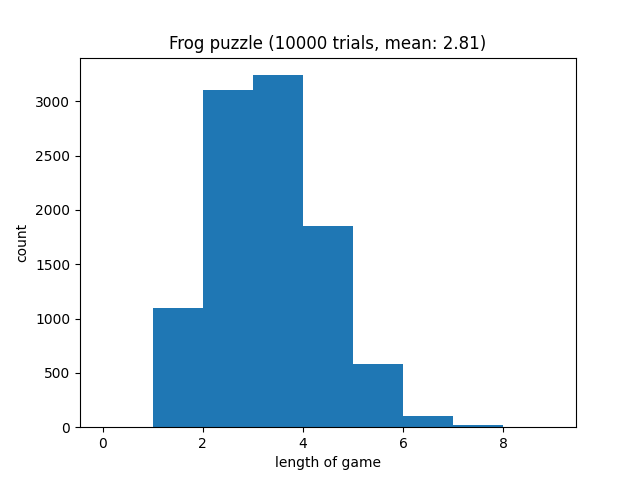
\includegraphics[width=.5\textwidth]{frog_puzzle_histogram.png}
%	\caption{Histogram showing the number of transitions to complete ``frog puzzle" for 10000 trials.}
%	\label{frog_puzzle}
%\end{figure}

\end{document}
